\section{Data}\label{sec:data}
Working versions of encoder and decoder scripts are available at \url{https://github.com/trstephen/elec483}.
The scripts will embed and extract a text watermark from a provided grayscale or color image.
Figure~\ref{fig:wm} shows the effect of adding a watermark to an image.

\begin{figure}[htpb]
  \centering
  \subfigure[Original]
  {
    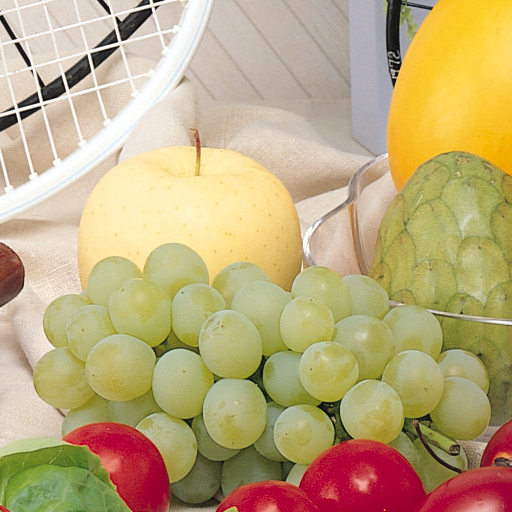
\includegraphics[width=0.475\linewidth]{graphics/fruits}
  }
  \subfigure[Watermarked]
  {
    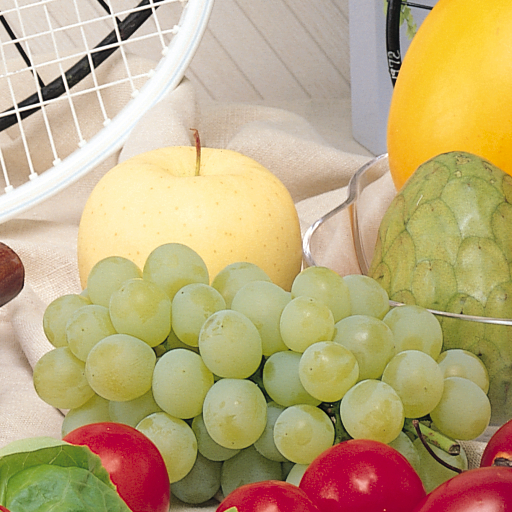
\includegraphics[width=0.475\linewidth]{graphics/fruits_wm}
  }
  
  \caption{A 22 character watermark has been embedded in the Y layer of the image}
  \label{fig:wm}
\end{figure}

To evaluate the effects on image quality  with spatial and frequency alterations, we compared the method described in Section~\ref{sec:impl} to one that embeds the binary sequence without the BCH code directly in the image grayscale values.
This spatial embedding method produced a PSNR of 49.3924, significantly less than the PSNR of 58.7447 with our frequency embedding method.
The frequency embedding method performs better because each message bit is encoded in a block of 64 pixels, rather than concentrated into single pixel.
Additionally, the relative change in value from embedding a bit is smaller in the frequency domain.

We also attempted to determined the best ``layer'' to embed the watermark in a color image.
We used a couple test color images, each with RGB and YCbCr\footnote{Subsampled with 4:4:4 BT.601 standard.} encoded variants.
The process in Section~\ref{sec:enc} was altered slightly to embed the watermark in a single layer and reconstruct the watermarked image using the watermarked layer and two unaltered layers.
In addition to the PSNR, which measures errors in the image component values, we computed the Structural Similarity Index (SSIM) which measures changes to image luminance, contrast and structure.
The SSIM is more predictive than PSNR for distortion as perceived by the human visual system \cite{Wang2004}.

The results in Table~\ref{tbl:color-psnr} show that embedding a watermark in any RGB layer causes less of a decrease in PSNR and SSIM than embedding it in any YCbCR layer.

\begin{table}[htpb]
  \centering
  \caption{Effects on PSNR after embedding a watermark in a single layer}
  \label{tbl:color-psnr}
  \begin{tabular}{@{}lcll@{}}
    \toprule
    \multicolumn{1}{c}{Source Image} & Layer & \multicolumn{1}{c}{PSNR}  & \multicolumn{1}{c}{SSIM}   \\
    \midrule
    \multirow{3}{*}{peppersYCbCr}
       & Y   & 58.91533 & 0.99997 \\
       & Cb  & 58.12800 & 0.99996 \\
       & Cr  & 58.95000 & 0.99996 \\
    &  &  \\
    \multirow{3}{*}{peppersRGB}
       & R   & 63.60164 & 0.99999 \\
       & G   & 63.74127 & 0.99999 \\
       & B   & 63.70763 & 0.99999 \\
    &  &  \\
    \multirow{3}{*}{fruitsYCbCr}
      & Y   & 58.88691 & 0.99988 \\
      & Cb  & 57.95389 & 0.99983 \\
      & Cr  & 59.07317 & 0.99987 \\
    &  &  \\
    \multirow{3}{*}{fruitsRGB}
      & R   & 63.88637 & 0.99995 \\
      & G   & 63.69708 & 0.99997 \\
      & B   & 63.59464 & 0.99995 \\
    \bottomrule
  \end{tabular}
\end{table}

The decrease in SSIM for watermarks embedded in the Y layer is not surprising since luminance is weighted in the SSIM value.
This explains the better SSIM for RGB embedding since the luminance is a weighted sum of all RGB layers.
However, the same decrease also occurs when the watermark is embedded in the chrominance layers even though chrominance changes are not measured directly by SSIM.

The effect of luminance changes on SSIM values does not explain why RGB embedding also has a better PSNR.
This behavior is counterintuitive and warrants further research.

